\noindent \textbf{Dear SIGMOD Chair and Referees:}

We thank the reviewers for the helpful feedback on our paper. We addressed all of the concerns and clarified the questions and conclude the major modifications as follows:
\begin{enumerate}
\item We clarified our scalability statement in and extend our experiments in Figure~\ref{f:attr100}. We demonstrated that even with the most complex setting, \texttt{UPDATE} queries with \textit{range} \texttt{WHERE} clause, \sys scales to databases with $100k$ records when the corruption age is as old as $250$. 
\item We demonstrated that we are able to simulate errors with different complexity by manipulating parameters in our synthetic data generator. As mentioned by the reviews, the complexity of errors (a.k.a. harness of the problem) could be measured by the level of query interactions. In our revision, we included references to existing experiments that study \sys's performance over the level of query interaction (R4) and also conducted additional experiment that investigate \sys's performance over \textit{query selectivity} in R3.5. 
\item We explained why \sys distinguishes from existing works on identifying tuples in data source that are ``responsible'' to errors in \texttt{SELECT} query results. We included extensive analysis in R3.5 explaining all suggested baseline comparisons in the review and proved that none of them could solve the problem addressed by \sys. 
\item We clarified all the assumptions in Section~\ref{sec:abstractions} and misleading definition in Section~\ref{sec:opt:query} (Definition~\ref{eq:dependency}) and the \textit{Big-M} assignment in Section~\ref{sec:linearize}.
\end{enumerate}

\subsection*{Meta Review Details}
\noindent \textbf{R1: Discuss and clarify the soundness of slicing techniques.} 

We propose tuple, query, and attribute-slicing optimization to improve \sys's performance. 

Tuple-slicing optimization is primary applied on fixing workload with range predicates. The probability of making an incorrect log repair due to tuple-slicing is very low: A failure case only happens when there exists a different set of queries (other than the actual incorrect queries) in the workload that modifies every tuple in the complaint set. In fact, the probability of having such a case in our synthetic datasets is lower than 0.001\% but could be higher with less attributes in the database and fewer tuples. For workloads with point predicates (a.k.a only a small set of tuples---$1-2$ are updated by each individual query), including most benchmark workloads, with the help of other optimization, queries that might result in a incorrect repair are already pruned ahead , thus applying tuple-slicing is most likely to be correct. In summary, tuple-slicing is an effective method to improve the performance of the basic approach, without compromising, and often improving, repair quality.

Attribute-slicing and query-slicing remove irrelevant attributes and queries according to whether or not they would affect the incorrect values in the complaints, thus they are guaranteed to be correct. 

\noindent \textbf{R2 Clarify the assumptions, their interaction, and why they are realistic in practice. clarify that the system is not repairing the update queries, but the affected data (i.e., query is not correct and errors can still happen).} 

We summarize all assumptions in Section~\ref{sec:abstractions} 

\noindent \textbf{R3 Add experiment with larger data size, or clarify why they cannot be done.}

We extend our experiment with larger database sizes in Figure~\ref{f:attr100} with up to $100k$ tuples. 

\noindent \textbf{R4 Investigate how many of the errors exhibit interesting patterns (such as a later update masking the effect of an earlier erroneous one). If there are already lots of examples of this, compare effectiveness on the "simple" errors with the "complex" ones; otherwise, you should improve the test data generator.}

To carefully evaluate \sys's performance over problems with different properties, we introduce a synthetic data generator in Section~\ref{sec:setup} with multiple adjustable parameters, including query type, workload and database size, and query selectivity. 
With the help of these parameters, we are able to control one of the key properties in the workload, the interaction of the queries, 
and thus to better understand \sys's performance. The level of query interactions greatly influences to the hardness of the problem as errors may propagate differently under different scenarios. 

There are many factors that may affect the level of query interactions. In general, \texttt{UPDATE} queries are heavily interact with each other than \texttt{INSERT} or \texttt{DELETE} queries since tuples persist in the database and may be continuously updated by the following \texttt{UPDATE} queries. We demonstrate this in Figure~\ref{f:indelup_time} and observe that under the same corruption age, \texttt{UPDATE}-workload requires longer time to solve than \texttt{DELETE} and \texttt{INSERT}-workloads. For \texttt{UPDATE} queries, \textit{constant} \texttt{SET} clauses do not require former attribute value(s), and thus have less query interaction compare to queries with \textit{relative} \texttt{SET} clauses (Figure~\ref{f:qidx_time}). Under default parameters, \texttt{UPDATE} queries with \textit{point} \texttt{WHERE} clauses update less amount of tuples than queries with \textit{range} \texttt{WHERE} clauses. Thus, the first type oftentimes has lower level of query interaction and easier to solve in practice (Figure~\ref{f:qidx_time}). For \texttt{UPDATE} queries with \textit{range} \texttt{WHERE} clauses, we found that both the number of attributes $N_a$ and query selectivity $s$ may strongly influence the level of query interaction (refer to R3.5 for details). Under our default setting, increase the number of attribute $N_a$ reduces the query interaction and thus we observe that problems with larger number of $N_a$ are easier to solve in Figure~\ref{f:attr}. On the other hand, increasing query selectivity $s$ means more tuples are updated by each query and thus leads to higher level of query interaction (demonstrated in R3.5).


\noindent \textbf{R5 Implementation of a baseline (described in the review) or explain why such baselines would fail in the context, to convince readers that complex patterns can be handled only by this new system.}

In this paper, \sys solves two problems: 1. it finds the root reason(s) in the query history that causing database errors, and 2. it fixed the incorrectness by proposing a query log repair. Existing works~\cite{Wu13, roy2014formal, chalamalla2014,meliou2011tracing} mentioned by reviewer 3 study highly corrected problems: in general, they all target at explaining erroneous or undesired query results by tracing back data source input and reporting either particular input tuples or common input patterns. After carefully analysis, we conclude that none of these existing works could fix the incorrect queries (problem 2) nor solve the error identification task (problem 1) effectively and efficiently. Please refer to R3.2 for details.


\subsection*{Reviewer 1 Details}
\noindent \textbf{R1.1 What are the soundness/correctness properties needed for the slicing heuristics to be applicable/useful? It seems they can be useful even if not sound, but showing this is the case on non-synthetic data would help. I appreciate that realistic benchmarks may not be available though.}

(Refer to R1)

\noindent \textbf{R1.2 Please correct definition 6.} \xlw{Original def. 6 seems misleading, let's verify it.}

The \textbf{full-impact}, $\mathcal{F}(q_i)$, of a query $q_i$ includes all attributes that may modified by the query $q_i$ and it is calculate by the intermediate-impact of all its consecutive queries. Let us denote $\mathcal{F}_j(q_i)$ as the intermediate-impact of query $q_i$ on query $q_j$ ($j > i$) and $\mathcal{F}_j(q_i)$ is defined as follows.
 \[
    \mathcal{F}_j(q_i)=\mathcal{F}_{j-1}(q_i)\bigcup_{\substack{\mathcal{F}_{j-1}(q_i)\cap \mathcal{P}(q_j) \neq \emptyset}} \mathcal{I}(q_j),
 \]
With initial impact $\mathcal{F}_i(q_i)  = \mathcal{I}(q_i)$. The full-impact of $q_i$, $\mathcal{F}(q_i)$ is indeed the impact on the final query $q_n$, $\mathcal{F}_n(q_i)$. For example, in the following query log:\\
\textit{q1 writes t.A; \\
q2 reads t.A and writes u.B; \\
q3 reads u.B and writes v.C.}\\
\[\mathcal{F}_1(q_1) = \{t.A\};\] 
\[\mathcal{F}_2(q_1) = \{t.A\} \bigcup_{\mathcal{F}_1(q_1) \cap \{t.A\} \neq \emptyset} \{u.B\} = \{t.A, u.B\};\]
\[\mathcal{F}_3(q_1) = \{t.A, u.B\}\bigcup_{\mathcal{F}_2(q_2) \cap \{u.B\} \neq \emptyset} \{v.C\} = \{t.A, u.B, v.C\}.\]
Thus the full-impact of $q_1$ is $\{t.A, u.B, v.C\}$.

\noindent \textbf{R1.3 Do the experiments substantiate the claim of scalability to "large" databases of 100k records? If so the experimental evaluation needs to explain this more clearly. If not the introduction must avoid overselling this point.}

We evaluate performance of \sys compare to a heuristic approach on databases of $100k$ records (in Appendix~\ref{sec:heuristic}) and further extend our experiment in Figure~\ref{f:attr100} to databases with $100k$ records. 

\noindent \textbf{R1.4 It's also not entirely clear why it is correct to use a "large/unused" value $M^+$ for attributes of deleted tuples. Please spell this out.}

For clarification we rename the former variable $M^+$ as $M^-$ to distinguish from $M$ and emphasis its relationship with $M$ as $M^- \leq M$. 
$M^-$ is set to a large enough number outside the attribute domain in order to guarantee that \sys would fix the incorrect \texttt{DELETE} query instead of its consecutive \texttt{UPDATE} queries. Recall our MILP encoding in Equation 6, to ensure that the attribute value of tuple is set to $M^-$ in a \texttt{DELETE} query, one need to set $x_{q_i,t} = 1$ which only requires variable adjustment in the \texttt{WHERE} clause such that $\sigma_{q_i}(t) = 1$. Alternatively, it may also feasible to manipulate the consecutive \texttt{UPDATE} query such that the \texttt{SET} clause updates the tuple to $M^-$ as $\mu_{q_i}(t) = M^-$ (according to Equation 4). Modifying \texttt{DELETE} query or \texttt{UPDATE} query may all lead to feasible solution, however, different objective-function values are associated with them. By setting $M^-$ to a ``sufficiently large'' number, we force the objective-function value of the \texttt{UPDATE} query modification exceedingly large than the \texttt{DELETE} query's. Thus it is  guaranteed that \sys will always fix the incorrect \texttt{DELETE} query instead of its consecutive \texttt{UPDATE} queries. In addition, we set $M^- \leq M$ to avoid generating infeasibility conditions.

\subsection*{Reviewer 2 Details} \xlw{Reviewer 2 does not request any significant revision. These are listed as weak point.}

\noindent \textbf{R2.1 Given that the paper considers a novel problem, I believe it could trigger quite some follow-up work. However, to do so, I personally think that further technical details or detailed theoretical discussion are necessary. }

(add text)

\noindent \textbf{R2.2 I find the experimental evaluation rather preliminary and would appreciate experiments on larger data sets or some real data set.}

(add text)
\subsection*{Reviewer 3 Details}

\noindent \textbf{R3.1 The problem is indeed difficult with several sources of complexity. It is challenging to find the right setting to handle it and assumptions must be put in place to solve it with some degree of confidence. However, right now assumptions are scattered all around the paper, and some of them should probably be revised.
My first suggestion is to collect all the restrictions or hypothesis in a unified discussion and try to assess how close is the ultimate setting to the real world scenarios.} 

{Refer to R2}

\noindent \textbf{R3.2 Errors are indeed in the queries, but are ultimately data errors that are considered here (no structural errors in the query). It seems related, existing solutions~\cite{Wu13, roy2014formal, chalamalla2014,meliou2011tracing} can be directly applied by modelling the query data as source data + SELECT queries. In fact, queries data can be modelled as sources with a new attribute representing the query id, and the data in this papers is the view in previous work. Once identified the problems in the view (as done in all papers) evidence can be carried back to the sources and mined to find the explanations. If the errors are coming from one query (as assumed in most of the exp in this work), I am confident the query attribute will be identified and the explanation will point to that query. I understand that the implementation of such baselines may go behind the scope of the revision, but I believe it would be great if the author can precisely explain why such baselines would fail in their context. ( i suspect the reason is discussed in point 5). }

In this paper, \sys solves two problems: 1. it finds the root reason(s) in the query history that causing database errors, and 2. it fixed the incorrectness by proposing a query log repair. Existing works mentioned above study highly corrected problems: in general, they all target at explaining erroneous or undesired query results by tracing back data source input and reporting either particular input tuples or common input patterns. After carefully analysis, we conclude that none of these existing works could fix the incorrectness nor solve the error identification task effectively and efficiently. 

In order to use these works to diagnose query history, we first convert the \textsc{Optimal Diagnosis} problem in Definition 4 as \textsc{Source data + SELECT queries} problem:
Given database states $D_0$ and $D_n$, a query log $\mathcal{Q} = \{q_i\}$ such that $\mathcal{Q}(D_0) = D_n$, and a desired database state $D_n^*$ with no errors, we model the \textsc{Source data + SELECT queries} problem by creating a table $P$ for under-determined parameters in $\mathcal{Q}$ and table $D_0$ as source tables; and a single nested SELECT query $q_n'$ for queries in $\mathcal{Q}$. We demonstrate an abstract example in Example~\ref{fig:example}.
\begin{figure}[t]
The \textsc{Optimal Diagnosis} problem:\\
    \begin{minipage}[t]{0.1\textwidth}
         \vspace{0pt} 
         \centering
        \begin{tabular}{ll}
            \multicolumn{2}{l}{Table $D_0$}\\
            \toprule
            \textbf{A}  & \textbf{B}\\
            \midrule
			 1 & 1 \\
			 2 & 2 \\
			 3 & 5 \\
            \bottomrule
            \\
        \end{tabular}
    \end{minipage}
    \begin{minipage}[t]{0.2\textwidth}
         \vspace{0pt} 
         \centering
        \begin{tabular}{p{26ex}}
            \multicolumn{1}{l}{\emph{Query log}: $\mathcal{Q}$}\\
            $q_1$: \texttt{\small UPDATE T SET B=B+1}\\
            \texttt{\small WHERE A > 2 and a < \sout{5} {\color{red} 3}} \\
            $q_2$: \texttt{\small UPDATE T SET B=B+3}\\
                  \texttt{\small WHERE A > 0 and a < 4} \\
        \end{tabular}
    \end{minipage}
    \begin{minipage}[t]{0.16\textwidth}
         \vspace{0pt} 
         \centering
        \begin{tabular}{ll}
            \multicolumn{2}{l}{Table $D_2^*$}\\
            \toprule
            \textbf{A}  & \textbf{B}\\
            \midrule
			 1 & 1 \\
			 2 & 2 \\
			 3 & {\textbf{6}} \\
            \bottomrule
            \\
        \end{tabular}
    \end{minipage}
The \textsc{Source data + SELECT queries} problem: \\
\begin{minipage}[t]{0.1\textwidth}
         \vspace{0pt} 
         \centering
        \begin{tabular}{ll}
            \multicolumn{2}{l}{Table $D_0$}\\
            (same as above) \\
        \end{tabular}
    \end{minipage}
\begin{minipage}[t]{0.36\textwidth}
         \vspace{0pt} 
         \centering
        \begin{tabular}{llllll}
            \multicolumn{6}{l}{Table $P$}\\
            \toprule
            \textbf{$p_1$}  & \textbf{$p_2$} & \textbf{$p_3$} & \textbf{$p_4$}  & \textbf{$p_5$} & \textbf{$p_6$} \\
            \midrule
			 1 & 2 & 3 & 3 & 0 & 4\\
            \bottomrule
            \\
        \end{tabular}
    \end{minipage}\\
        \begin{minipage}[t]{0.22\textwidth}
         \vspace{0pt} 
         \centering
        \begin{tabular}{p{2ex}p{55ex}}
         \multicolumn{2}{l}{\emph{Queries}: }\\
        $q'_1$: &
        \texttt{\small SELECT $D_0.A$ AS A, $D_0.B$+$p_1$ AS B FROM $P, D_0$ } \\
        & \texttt{\small WHERE $D_0.A$ > $p_2$ AND $D_0.A$ < $p_3$ UNION ALL}\\
        & \texttt{\small SELECT $D_0.A$ AS A, $D_0.B$ AS B FROM $P, D_0$ }\\
        &\texttt{\small  WHERE $\neg$($D_0.A$ > $p_2$ AND $D_0.A$ < $p_3$)} \\
        $q'_2:$ &
         \texttt{\small SELECT $D_1.A$ AS A, $D_1.B$+$p_4$ AS B FROM $P, q_1'\ as\ D_1$ } \\
        & \texttt{\small WHERE $D_1.A$ > $p_5$ AND $D_1.A$ < $p_6$ UNION ALL}\\
        & \texttt{\small SELECT $D_1.A$ AS A, $D_1.B$ AS B FROM $P, q_1'\ as\ D_1$ }\\
        &\texttt{\small  WHERE $\neg$($D_1.A$ > $p_5$ AND $D_1.A$ < $p_6$)} \\
        \end{tabular}
    \end{minipage}
    \caption{An abstract example for R3.2. (For simplicity, we use $q_1'$ for the input sub-query when introducing $q_2'$.)}
\label{fig:example}
\end{figure}

\noindent \textbf{[Roy et al. SIGMOD 2014, Wu et al. VLDB 2013, Chalamalla et al. SIGMOD 2014]} \\
TLDR: These papers quantify responsibility of input data to errors in the output, however responsibility


These papers focus on detecting and summarizing the likely source tuples by propagating ``responsibility'' from annotated output error tuples to sources. ~\cite{Wu13} targets at explaining a set of SELECT query results by a conjunction of predicates on attributes where the SELECT clause in each query is restricted to a single aggregate operator. 
Similarly, ~\cite{roy2014formal} explains a group-by SQL query with a single aggregate function. Since there is no obvious mapping between complaints and a particular aggregate function, both algorithms cannot solve the error identification problem. Instead of aggregation results, ~\cite{chalamalla2014} searches for explanations for data quality rule violations. Even though complaints can be expressed as data quality rules, the algorithm does not distinguish the actual input source error (in $D_0$) and query parameter error (in $P$). Thus, in Example~\ref{fig:example}, the explanation $D_0.A = 3$ on table $D_0$ is also a valid explanation. Thus, this work cannot effectively solve the error identification problem either.

\noindent \textbf{[Meliou et al. SIGMOD 2011]} \\
TLDR: The number of disjunctions in the generated SAT expression increases exponentially with respect to the number of queries in the log.  For instance, if the database contained 100 tuples and 10 queries, the number of disjunctions would be $\cdot 2^{10}$ and thus the number of lineage expressions would be $100\cdot 2^{100}$.

The View-Conditioned Causality(VCC) work takes a set of input variables $\mathbf{X}$, a transformation $\mathbf{\Phi} =\{\Phi_1, ... , \Phi_m\}$ computing the
output values $\mathbf{z}$, and a ground truth $\hat{\mathbf{z}}$, and detects input variables that are responsible for data errors $\mathbf{z}|\hat{\mathbf{z}}$. 
The \textsc{Source data + SELECT queries} problem can be expressed as a VCC problem where cells in $P$ form the input variables $\mathbf{X}$ and each tuple $t_i$ in $D_0$ and the SELECT query $q_n'$ is translated into a lineage expression $\Phi_i$. In each lineage expression $\Phi_i$, tuple values in $D_0$ and $D_n^*$ are further converted into constant variables. By doing so, only variables in $P$ will be selected to explain data errors. In Example~\ref{fig:example}, lineage expression $\Phi_3$ for tuple $t_3$ is as following:
{\small
\begin{eqnarray*}
&((3 > p_2 \wedge 3 < p_3) \wedge (3 > p_5 \wedge 3 < p_6) \wedge (5 + p_1+p_4 = 6)) &\\
&\vee ((3 > p_2 \wedge 3 < p_3) \wedge \neg(3 > p_5 \wedge 3 < p_6) \wedge (5 + p_1= 6))& \\
&\vee (\neg(3 > p_2 \wedge 3 < p_3) \wedge (3 > p_5 \wedge 3 < p_6) \wedge (5 + p_4= 6))& \\
&\vee (\neg(3 > p_2 \wedge 3 < p_3) \wedge \neg(3 > p_5 \wedge 3 < p_6) \wedge (5 = 6))&
\end{eqnarray*}
}
Each row corresponding to the satisfactory condition for where clauses in $Q$. The first row, for example, means the where condition is true for both $q_1$ and $q_2$. The ground truth output values for $\mathbf{\Phi}$ are all set to \textit{True}. By solving the VCC problem, one can identify incorrect parameters in the query log. However, as you may notice, the lineage expressions for tuples in $D_0$ are composed by disjunctive sub-expressions with exponential cardinality to the number of queries in $Q$. Since the execution efficiency is highly correlated to the complexity of lineage expressions, VCC solves the error detection task but cannot solve it efficiently. 

To conclude, none of these highly correlated works could handle both problems addressed by \sys: ~\cite{meliou2011tracing} solves the error detection problem with low efficiency; ~\cite{chalamalla2014} may solve the error detection problem but fail to distinguish data source errors and query errors; ~\cite{Wu13} and ~\cite{roy2014formal} restricted to aggregations, thus cannot solve either problems.

\noindent \textbf{R3.3 Most of the technical contributions are on the scalability aspect, but relatively small datasets are tested. I suggest to explicitly test the scalability until the bottlenecks of the solutions become clear (the MILP module?)}

We extend our experiment with larger database size in Figure~\ref{f:attr100} and observe that with all optimization, \sys requires $~300$ sec to solve problems with $100k$ tuples and a corruption age of $250$ queries. 

\noindent \textbf{R3.4 I cannot grasp from the experiments section if the authors are counting the number of errors correctly identified or correctly fixed. Usually these are considered two different metrics in data repair. For example, given the problem of income >= 85700, do they consider it correctly fixed with any value that lead to repair of the identified problems or they require to get exactly 87500? 
I believe it must be the former as I don't see how they can always recover the correct value in general. If this is the case, this clearly explain the big drop in precision and recall when the complain set is incomplete. Unfortunately this implies that even complete complain sets do NOT guarantee that the query is correctly fixed and future errors will not occur (e.g. the system may discover 87200 as the correct fix, it covers all case, but it does not cover new data)}

In our experiment, we measure \sys's accuracy as whether all complaints are correctly fixed. In the example, we also consider $income >= 87200$ as a correct query repair as it resolves all the reported complaints. In addition, the repaired query is allowed to differ from the true query. However, this is very rare in practice and we show that \sys always pick the correct query to fix when the complaint set is complete. Though \sys dos not guarantee to propose a query log repair that is exactly the same with the original true query log, it identifies the incorrect query and provides a reasonable suggestion of how to fix the problem. 

\noindent \textbf{R3.5 I believe the way that errors are introduced can be improved. Randomly introducing errors do not guarantee that complex patterns (such as the one in Figure 1) happen in the test datasets. In fact, what make the problem challenging is the interaction of the queries. I suggest to have an experiment where this interaction is enforced in the noise injection so that the approach can really show its power wrt to simpler techniques (such as point 2 above). 
Unfortunately having some guarantee on the way that errors are introduced can be a challenging problem, a recent paper discusses this topic (Arocena et al, PVLDB 15).}
\begin{figure}[t]
\centering
  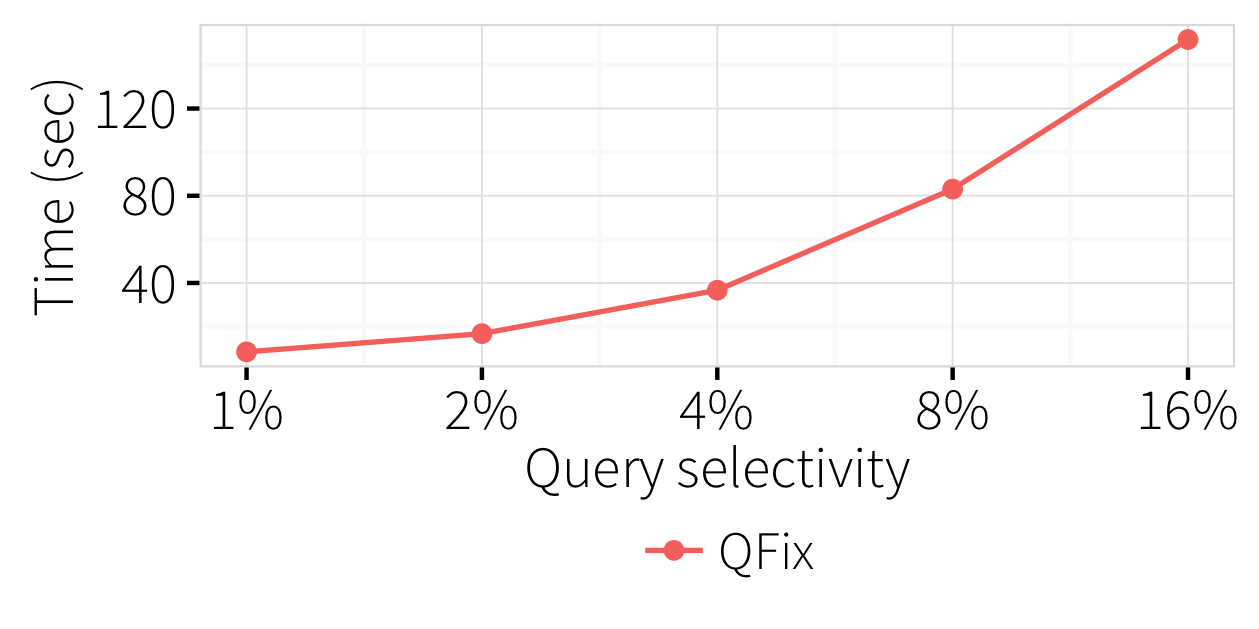
\includegraphics[width = \columnwidth]{figures/rangevstime}
 \caption{\sys on increasing }
  \label{f:selectivityvstime} 
\end{figure}
We introduce a synthetic data generator in Section~\ref{sec:setup} with multiple adjustable parameters, including
query type, workload and database size, and query selectivity, to simulate the workloads with diverse properties. 
With the help of these parameters, we are able to control one of the key properties in the workload, the interaction of the queries, 
and thus to better understand \sys's performance. 

In this section, we measure the interaction of queries as whether these queries update the same set of tuples and we further 
narrow down the query log size into two for simplification. For a \texttt{UPDATE}-only workload with \textit{range} \texttt{WHERE} clauses, 
the probability that two queries, $q_i$ and $q_j$, update a non-empty set of tuples is as as follows.
\begin{multline*}
Pr(q_i\cap q_j \neq \emptyset) =\\ 
Pr(\sigma_{q_i}.A= \sigma_{q_j}.A)Pr(q_i\cap q_j \neq \emptyset |\sigma_{q_i}.A= \sigma_{q_j}.A) \\
+ Pr(\sigma_{q_i}.A\neq \sigma_{q_j}.A)Pr(q_i\cap q_j \neq \emptyset |\sigma_{q_i}.A\neq \sigma_{q_j}.A), 
\end{multline*}
Where $Pr(\sigma_{q_i}.A= \sigma_{q_j}.A)$ is the probability that the \texttt{WHERE} clauses of two queries are on the same attribute with probability $\frac{1}{N_a}$
where $N_a$ is the number of attributes in the database. When two queries select tuples based on the same attribute, 
the probability of non-empty interaction is equivalent to the probability 
that their \texttt{WHERE} clause ranges intersect with each other. Thus, $Pr(q_i\cap q_j \neq \emptyset |\sigma_{q_i}.A= \sigma_{q_j}.A) = 2*s$, where
 $s$ is the query selectivity percentage. In addition, $Pr(\sigma_{q_i}.A\neq  \sigma_{q_j}.A) = \frac{N_a-1}{N_a}$ is the probability that the \texttt{WHERE} clauses
of $q_i$ and $q_j$ select different attributes.  Assuming tuple values are evenly distributed in arbitrary attribute, the number of tuples selected by each query is roughly $n = N_d \cdot s$ where $N_d$ is the number of tuples in the database. Thus, the probability that these two queries update at least one common tuple is $Pr(q_i\cap q_j \neq \emptyset |\sigma_{q_i}.A\neq \sigma_{q_j}.A) = 1 - \frac{C(N_d - n, n)}{C(N_d, n)}$ where $C$ is the \textit{Combinations function}\footnote{Combinations function: $C(n,r) = \frac{n!}{r!(n-r)!}$}. In conclude, the probability that two queries have non-empty interaction is estimated as follows.
\begin{multline} \label{eq:pr}
Pr(q_i\cap q_j \neq \emptyset) = \frac{2s}{N_a} + \frac{N_a-1}{N_a} \cdot (1 - \frac{C(N_d - n, n)}{C(N_d, n)}), 
\end{multline}
Where $n = N_d \cdot s$.

In Section~\ref{sec:experiments:dbproperties}, we study the influence of number of attribute $N_a$ on \sys performance (Figure~\ref{f:attr}) and observe that larger number of attributes requires less execution time with \sys with all optimization. This is expected since with the default parameter settings $Pr(q_i\cap q_j \neq \emptyset)$ is negative proportional to the number of attributes.

In addition to the number of attribute, we evaluate \sys performance over query selectivity $s$ in this section. According to Equation~\ref{eq:pr},  the probability that two queries interact with each other is $~0.31$ under default parameter settings and increases with the query selectivity $s$. As shown in Figure~\ref{f:selectivityvstime}, the execution time of \sys also increases with higher query selectivity or higher query interaction. 


\pagebreak